%% fancy header & foot
\pagestyle{fancy}
\lhead{[ELEC-H-2001] Électricité\\ LABO \no 1A : Circuits réactifs en régime - Phaseurs et impédances \ifthenelse{\boolean{corrige}}{~-- corrigé}{}}
\rhead{v1.0.0\\ page \thepage}
\cfoot{}
%%

\pdfinfo{
/Author (Renaud Theunissen et Youssef Agram, ULB -- BEAMS-EE)
/Title (Laboratoire 1A ELEC-H-2001, Circuits réactifs en régime - Phaseurs et impédances)
/ModDate (D:\pdfdate)
}

\hypersetup{
pdftitle={Labo 1A [ELEC-H-2001] Électricité : LABO 1A ELEC-H-2001, Circuits réactifs en régime - Phaseurs et impédances},
pdfauthor={Renaud Theunissen et Youssef Agram, ©2020 ULB - BEAMS-EE},
}

\setlength{\parskip}{0.5cm plus4mm minus3mm} %espacement entre §
\setlength{\parindent}{0pt}


\begin{document}

\tptitle{}{Séance 1A~: Circuits réactifs en régime - Phaseurs et impédances}
\section{But de la manipulation}
Le but de cette séance est de vous familiariser avec le matériel de laboratoire et de vous amener à développer une approche d'investigation des phénomènes liés aux circuits électriques étudiés dans le cours d'ELEC-H-2001.

Pour ce laboratoire vous aurez besoin des éléments suivants :
\begin{itemize}
    \item Votre PicoScope
    \item Les trois sondes (câbles BNC fournis dans le kit).
    \item Le protoboard
    \item Les résistances $R_e$, $R_i$ et $R_j$
    \item L'inductance $L$
    \item Le condensateur $C_i$
\end{itemize}

\section{Pré-requis}
Pour réaliser cette séance de laboratoire, il vous est recommandé de relire attentivement les sections du syllabus suivantes :
\begin{itemize}
    \item Section 4.3 - Adaptation d'impédance
    \item Sections 5.1 à 5.3 - Loi des mailles et utilisation
    \item Section 7.3 - Phaseurs
    \item Section 7.4 - Impédances et admittances
\end{itemize}

\newpage

\section{Préliminaire théorique}
Soit le circuit ci-dessous où $R_1 = 20k\Omega$, $R_2 = 30k\Omega$ et $R_3 = 50k\Omega$:
\begin{center}
\begin{figure}[h!]
    \centering
    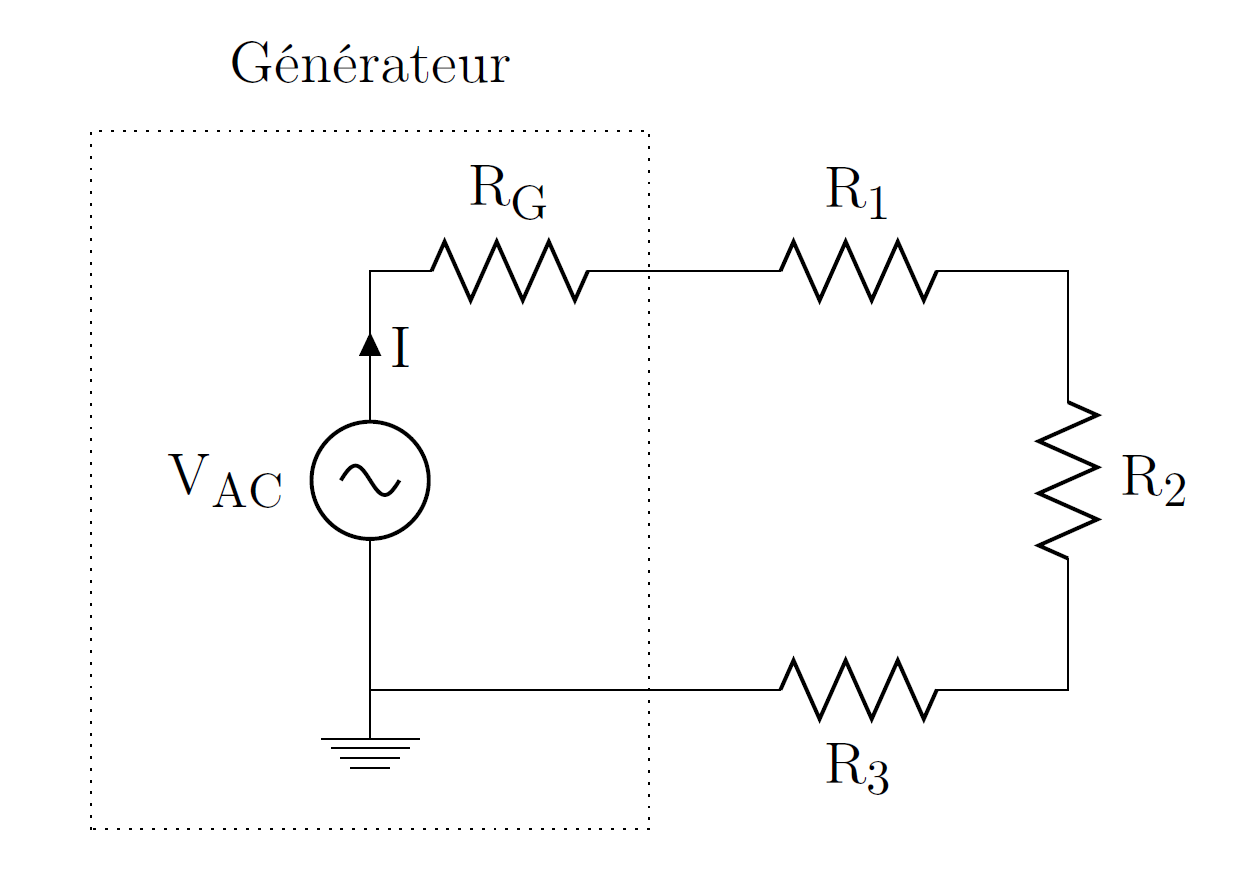
\includegraphics[scale = 0.7]{LABO1A/Ex1Lab1A.PNG}
    \caption{Circuit résistif}
    \label{fig:my_label}
\end{figure}
\end{center}
Si on impose une source $V_{AC}(t) = 10\sqrt{2} cos(2\pi 100t)$, on mesure à l'ampèremètre un courant efficace $I_{eff} = 0,1 mA$.

\subsection{Exercice 1}
\Question
{
\textit{Dans ce circuit, l'impédance de sortie $R_G$ du générateur peut-elle être négligée? Justifiez.}
}
{On observe dans la datasheet du Picoscope\footnote{https://www.picotech.com/oscilloscope/2000/picoscope-2000-manuals} que la résistance de sortie est de $600\Omega$.\\$R_G\ll R_{eq}=R_G+R_1+R_2+R_3=0.6+20+30+50=100.6 k\Omega$, donc $R_G\simeq 0.6\%R_{eq}$.\\
En réalité, la tension en sortie du générateur est donc de $10-0.6*0.1=9.94\ V$. Ceci n'est pas vraiment négligeable donc il est important d'en être conscient. Les résistances utilisées seront de même ordre de grandeur que celle de sortie du générateur. Il faudra donc le prendre en compte.}
\subsection{Exercice 2}
\Question
{
\textit{Vérifiez algébriquement la loi des mailles de ce circuit dans le domaine temporel.}}
{$$v_{AC}(t)=v_1(t)+v_2(t)+v_3(t)$$
$$\iff V_{AC_{eff}}\sqrt{2}\cos(2\pi100t)=(R_1+R_2+R_3)I_{eff}\sqrt{2}\cos(2\pi100t)$$
$$ \iff V_{AC_{eff}}=(R_1+R_2+R_3)I_{eff}=(20+30+50)\times 0.1 \longrightarrow OK$$}
\subsection{Exercice 3}
\Question
{\textit{Vérifiez la loi des mailles géométriquement dans le plan des phaseurs.}}
{La loi des mailles en phaseurs peut s'écrire $\underline{V_{AC}}=(R_1+R_2+R_3)\underline{I}$. Le circuit étant purement résistif, tous les signaux ont une phase nulle.
\begin{figure}[h!]
    \centering
    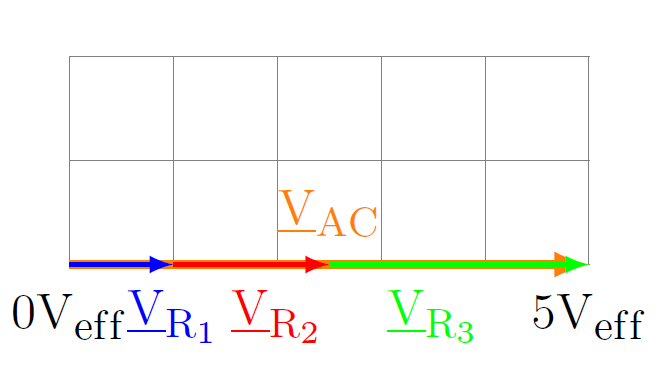
\includegraphics[scale=0.3]{LABO1A/plan_phaseur.PNG}
    \caption{Résolution dans le plan des phaseurs.}
    \label{fig:plan_phaseur}
\end{figure}}
\newpage
\section{Partie pratique}
\subsection{Réflexion analytique et physique}
Notre PicoScope dispose d'une résistance de sortie $R_G$. Si cette résistance est trop importante nous risquons d'avoir une réduction drastique de la tension du générateur.
\Question{
\begin{enumerate}
    \item Comment feriez-vous pour estimer la valeur de cette résistance de sortie ?\\
    \textcolor{darkblue}{L'idée est de connecter le générateur à une charge de résistance connue $R_e$. Ainsi, on pourra calculer la résistance $R_G$ à l'aide de la formule du diviseur résistif: $\underline{V_{AC}}=\frac{R_e}{R_e+R_G}\underline{V_{out}}$}
    \item Donnez la formule d'adaptation d'impédance (en phaseurs) en tension dans le cas où nous aurions un circuit du type :
    \begin{center}
        \begin{circuitikz}\draw
    (0,0)   to[sinusoidal voltage source, v=$v_G(t)$, i^>=$i_G(t)$] 
    (0,4)   to[resistor, l=$R_G$] 
    (4,4)   to[generic, l_=$Z_{charge}$, v^<=$v_{charge}(t)$]
    (4,0)--(0,0)   node[ground]{}
    ;
    \end{circuitikz}
    \end{center}\\
    \vspace{0.5cm}
\textcolor{darkblue}{Nous sommes en présence d'un diviseur résistif: $\underline{V_{G}}=\frac{R_G}{Z_{charge}+R_G}\underline{V_{charge}}$. $R_G$ doit donc être la plus faible possible afin de transmettre au mieux la tension à la charge.}
    \item Dans le cas où $Z_{charge}$ serait une résistance, que devrait valoir cette dernière pour que le module de $v_{charge}(t)$ soit égal à la moitié du module de $v_G(t)$?\\
    \textcolor{darkblue}{Elle devrait être égale à $R_G$}
\end{enumerate}}
{%C
}

\subsection{Mesures de signaux et interprétation - circuit résistif}
Réalisez sur votre \textit{Protoboard} le circuit suivant:
\begin{center}
    \begin{circuitikz} \draw
        (0,0) to[square voltage source, v=$v_{G}(t)$, i^>=$i(t)$] 
        (0,4) --
        (4,4) to[resistor, l_=$R_{i,j}$, v^<=$v_{R_{i,j}}$] 
        (4,0) to[resistor, l=$R_e$]
        (0,0) node[ground] {}
        ;
    \end{circuitikz}
\end{center}
\Question
{
Sachant que :
\begin{itemize}
    \item $R_e = 200\Omega$ 
    \item $v_G(t) = 2V$ et est une onde carrée de fréquence très basse ($f \approx 10Hz$)
    \item $R_G = 600\Omega$
    \item $R_{i,j}$ représente soit la résistance $R_i$ soit la résistance $R_j$ (il faudra tester les deux).
\end{itemize}
déterminez la valeur des résistances $R_i$ et $R_j$. \\
Vérifiez qu'en mettant les deux résistances $R_e$ en série avec les résistances $R_i$ et $R_j$ (donc pour obtenir une résistance équivalente $R_{tot}=R_e+R_e+R_i+R_j$) vous obtenez une tension $v_{R_{tot}}\approx 1V$.}
{En mesurant, la tension en sortie du générateur vaut $V_{in}=0.592\ V$ et la tension aux bornes de la résistance $R_i$ vaut $V_{R_i}=0.1289\ V$.\\
Pour $R_j$, la tension en sortie du générateur vaut $V_{in}=0.752\ V$ et la tension aux bornes de la résistance $R_j$ vaut $V_{R_j}=0.338\ V$. On obtient donc:
$$ R_i=\frac{-R_e\times V_{R_i}}{V_{R_i}-V_{in}}\simeq 55 \Omega$$ $$ R_j=\frac{-R_e\times V_{R_j}}{V_{R_j}-V_{in}}\simeq 163 \Omega$$}\\
En mesurant la tension aux bornes de tout le circuit nous obtenons le graphe suivant:
\begin{figure}[h!]
    \centering
    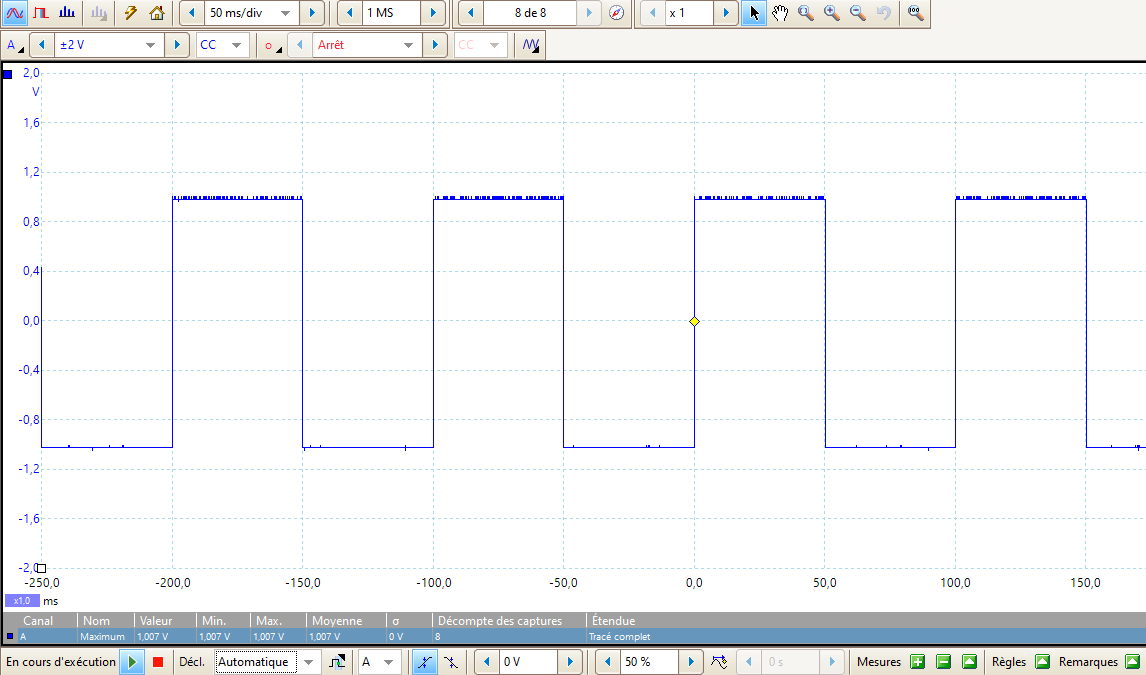
\includegraphics[scale=0.5]{LABO1A/Question_4_2_R.png}
    \caption{Tension aux bornes des 4 résistances}
    \label{fig:my_label}
\end{figure}

\newpage

\subsection{Réflexion analytique et physique}
Considérons le circuit suivant :
\begin{center}
    \begin{circuitikz} \draw
        (0,0) to[sinusoidal voltage source, v=$v_{G}(t)$, i^>=$i(t)$] 
        (0,4) to[resistor, l=$R_G$]
        (4,4) to[generic, l_=$Z_{charge}$, v^<=$v_{charge}(t)$] 
        (4,0) to[resistor, l=$R_e$]
        (2,0) to[resistor, l=$R_e$]
        (0,0) node[ground] {}
        ;
    \end{circuitikz}
\end{center}
Avec:
\begin{itemize}
    \item $v_G(t) = V_m sin(\omega t)$ la source de tension où $V_m = 2V$
    \item la fréquence $f = 50kHz$
    \item $Z_{charge}$ un composant réactif.
\end{itemize}

\Question{
\begin{enumerate}
    \item Quel dipôle devrions nous placer à la place de $Z_charge$ pour que la tension $v_{charge}(t)$ soit en avance de phase sur le courant $i(t)$?\\
    \textcolor{darkblue}{Nous devrions placer une inductance.}
    \item Quel dipôle devrions nous placer à la place de $Z_charge$ pour que la tension $v_{charge}(t)$ soit en retard de phase sur le courant $i(t)$?\\
    \textcolor{darkblue}{Nous devrions placer une capacité.}
    \item Si $Z_{charge}$ est un condensateur, comment doit évoluer la fréquence de la source si l'on veut augmenter le module de la tension $v_{charge}(t)$? Justifiez physiquement ce phénomène.\\
    \textcolor{darkblue}{Le diviseur impédant est en fait un filtre passe-bas. La capacité se comporte comme un circuit ouvert aux BF. Il faut donc que la fréquence soit la plus basse possible.}
    \item Si $Z_{charge}$ est une inductance, comment doit évoluer la fréquence de la source si l'on veut augmenter le module de la tension $v_{charge}(t)$? Justifiez physiquement ce phénomène.\\
    \textcolor{darkblue}{Le diviseur impédant est ici un filtre passe-haut. La capacité se comporte comme un court-circuit aux BF. Il faut donc que la fréquence soit la plus haute possible.}
\end{enumerate}}


\end{document}